\begin{figure*}[!t]
\centering
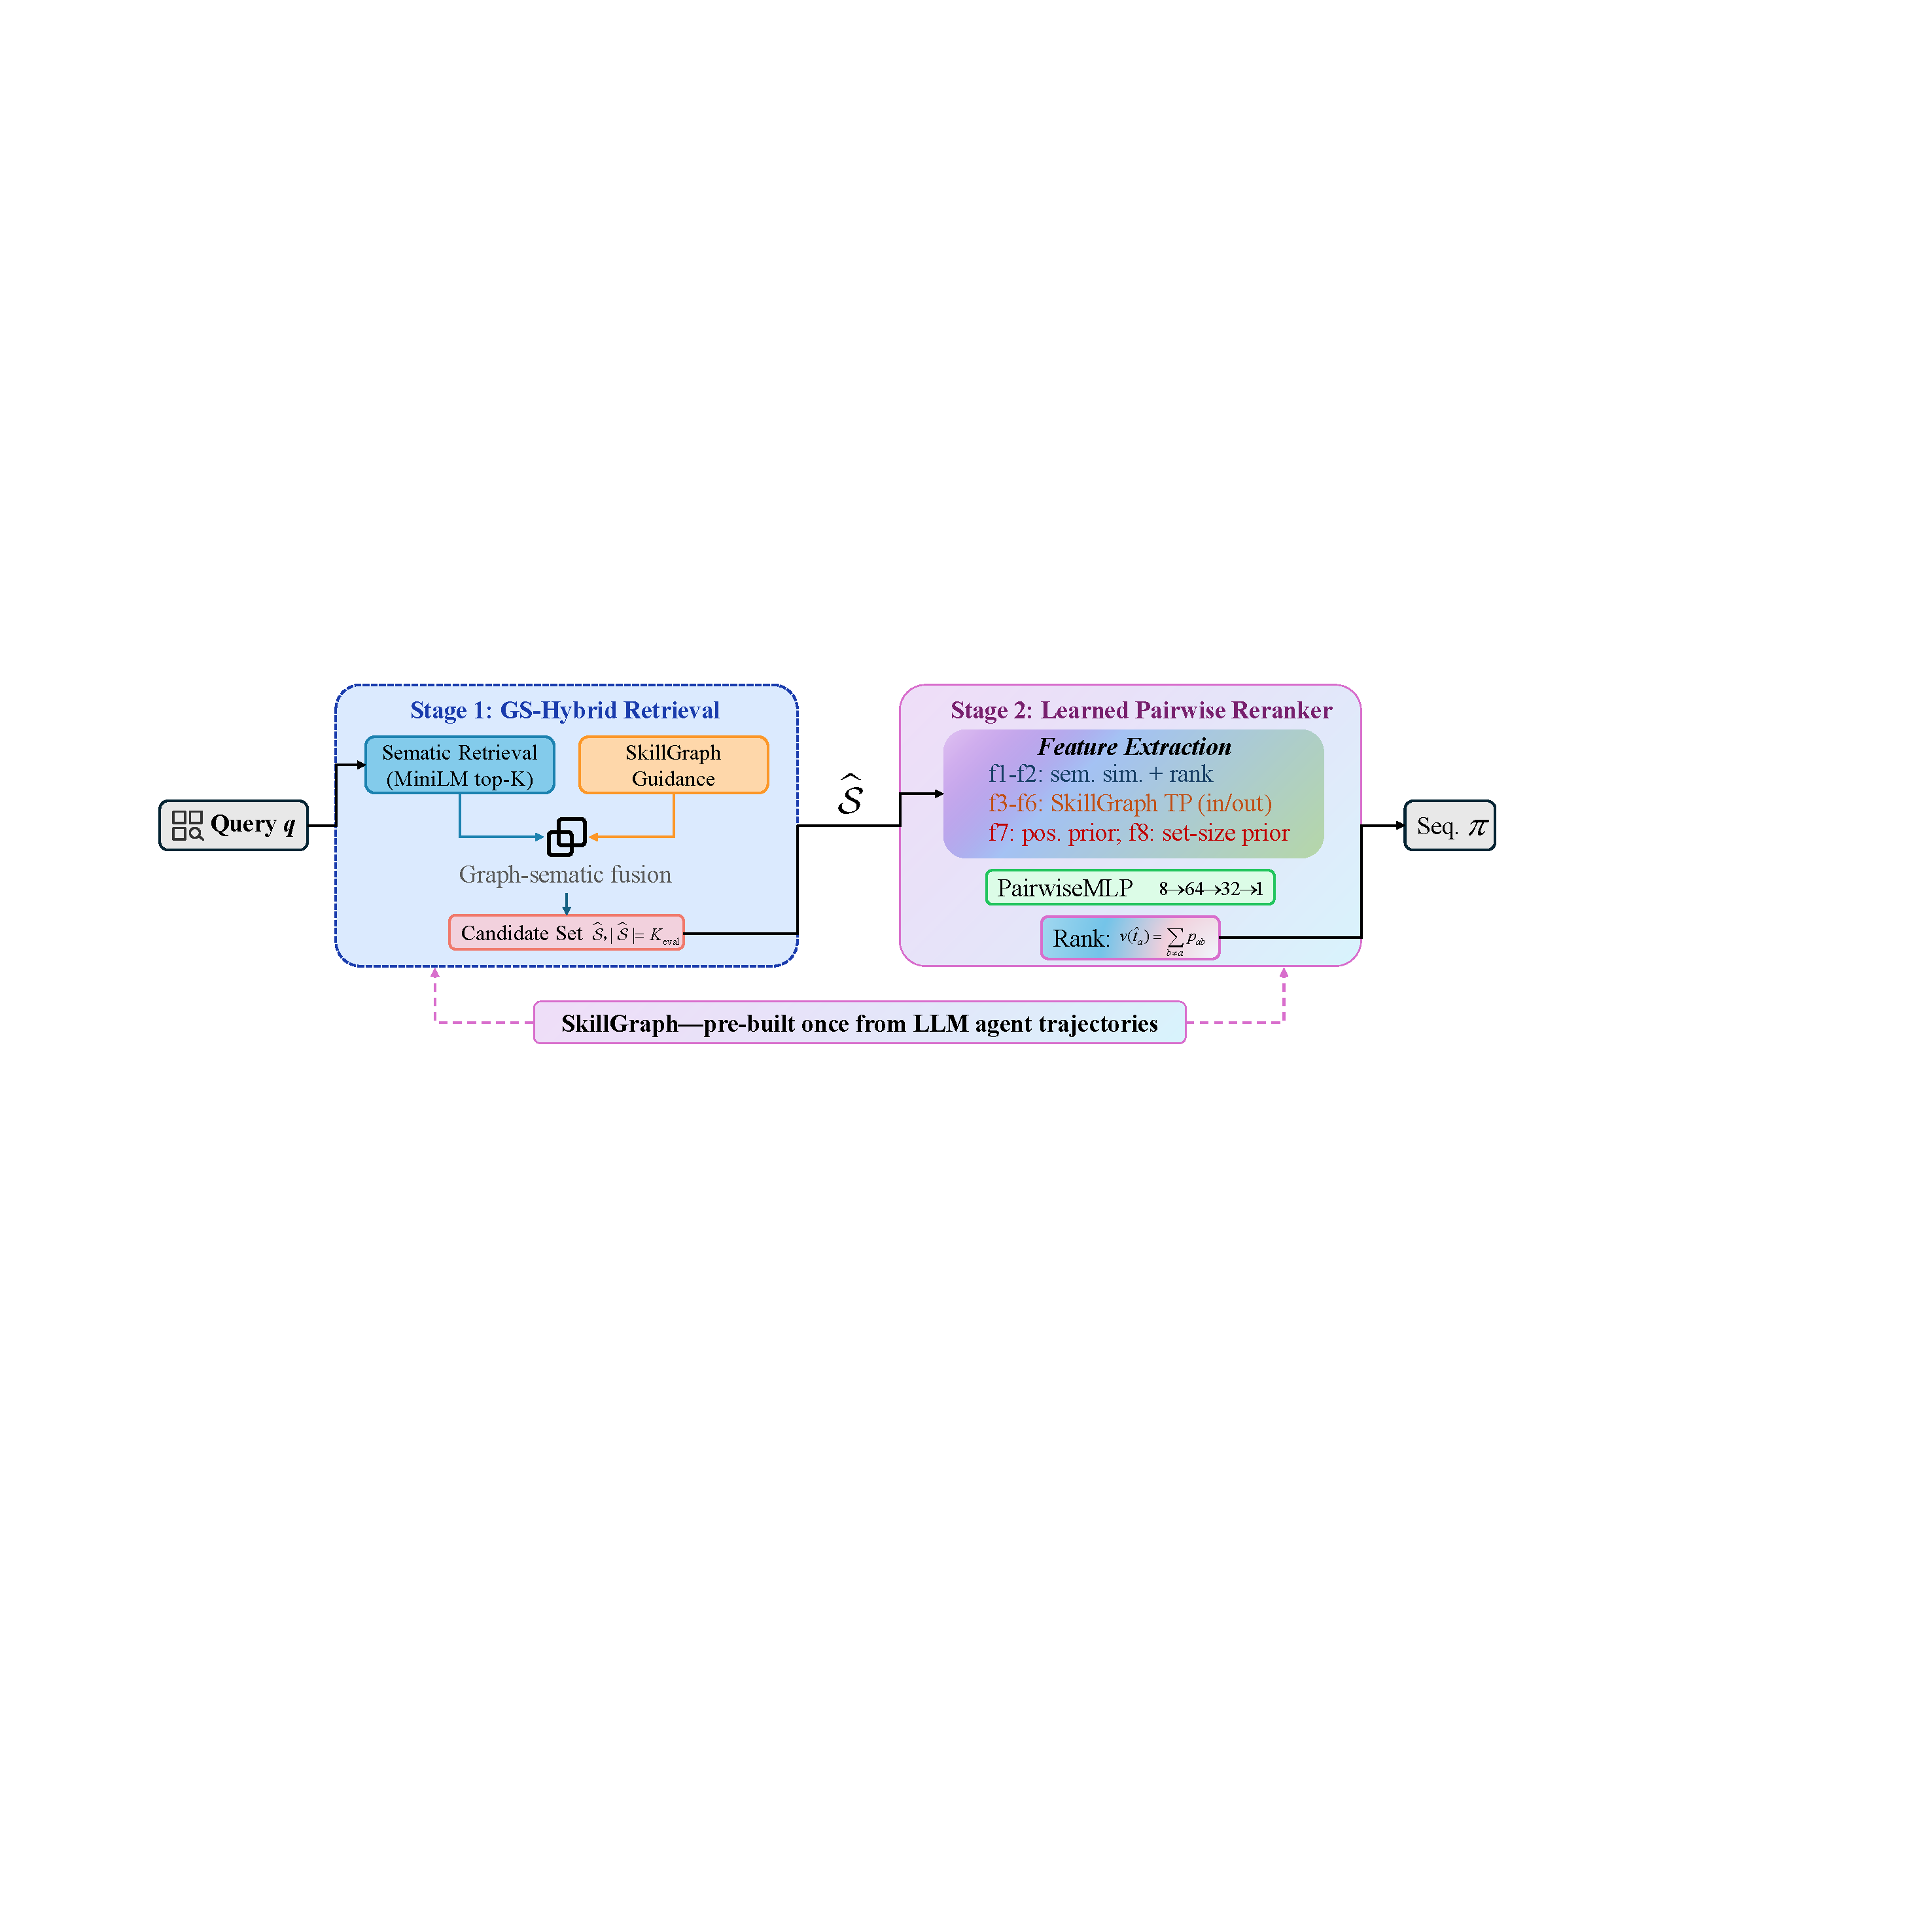
\includegraphics[
  width=\textwidth,
  trim=106.49bp 641.42bp 309.46bp 491.44bp,
  clip
]{figure/fig_framework_ppt.pdf}
\caption{Conceptual overview of the two-stage decoupled framework.
\textbf{Stage~1} (GS-Hybrid) constructs a candidate tool set $\hat{\mathcal{S}}$
of up to $K_{\mathrm{eval}}$ tools by combining dense semantic retrieval
with SkillGraph-guided candidate construction.
\textbf{Stage~2} (Learned Reranker) orders the candidates via a
PairwiseMLP that combines eight features: semantic similarity and rank
(f1--f2), SkillGraph transition probabilities (f3--f6), and positional
priors (f7--f8).
Decoupling the stages allows independent optimisation of set coverage
and sequence ordering, eliminating the single-stage selection-ordering
trade-off.}
\label{fig:framework}
\end{figure*}
